% !TeX document-id = {a7325568-63cb-46d1-95d6-777a45054e5a}
% !TeX TXS-program:compile = txs:///pdflatex/[--shell-escape]
\documentclass{article}
\usepackage{style}
\begin{document}
\maketitle
\tableofcontents
\section{Introducción}
El perceptrón es considerada la unidad básica para generar redes neuronales, esta puede clasificar vectores linealmente en dos categorías.
El objetivo del perceptrón es acercar a los vectores de entrada al patrón más cercano.
\newpage
\subsection{Modelo}
\begin{figure}[h!]
	\caption{Modelo}
	\centering
	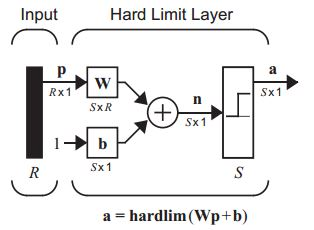
\includegraphics{model}
\end{figure}
\newpage
\section{Diagrama de Flujo}
\begin{figure}[htpb]
	\centering
	\includesvg[width = 400pt, height = 400pt]{diagram}
	\caption{Diagrama de Flujo}
\end{figure}
\newpage
\section{Resultados}
\subsection{Ejemplo 1}
\subsubsection{Datos}
\[p_1=
\begin{bmatrix}
2\\
2
\end{bmatrix}
, t=0
\]

\[p_2=
\begin{bmatrix}
1\\
-2
\end{bmatrix}
, t=1
\]

\[p_3=
\begin{bmatrix}
-2\\
2
\end{bmatrix}
, t=0
\]

\[p_4=
\begin{bmatrix}
-1\\
-1
\end{bmatrix}
, t=1
\]

\[W(0)= 
\begin{bmatrix}
 0.4121  & -0.9363
\end{bmatrix}
\]
$$ b= 0.2769 $$
\subsubsection{Resultado}
\begin{lstlisting}
W = 0.4121   -0.9363
b = 0.2769
Elija un modo: 1->Gráfico, 2->Regla de Aprendizaje
>>> 1
\end{lstlisting}
\begin{figure}[htpb]
	\centering
	\includesvg[width = 500pt, height = 500pt]{eg1}
	\caption{Gráfica del perceptrón 1}
\end{figure}
\newpage
\subsection{Ejemplo 2}
\subsubsection{Datos}
\[p_1=
\begin{bmatrix}
1\\
1
\end{bmatrix}
, t=0
\]

\[p_2=
\begin{bmatrix}
-1\\
-1
\end{bmatrix}
, t=1
\]

\[W(0)= 
\begin{bmatrix}
  -0.8946 &   0.4757
\end{bmatrix}
\]
$$ b= 0.2691 $$
\subsubsection{Resultado}
\begin{lstlisting}
W =  -0.8946    0.4757
b = 0.2691
Elija un modo: 1->Gráfico, 2->Regla de Aprendizaje
>>> 2
W = -0.2552   -0.6038
b = 0.4897
\end{lstlisting}
\begin{figure}[htpb]
	\centering
	\includesvg[width = 500pt, height = 500pt]{er1}
	\caption{Gráfica del perceptrón 2}
\end{figure}
\begin{figure}[htpb]
	\centering
	\includesvg[width = 500pt, height = 500pt]{er1v}
	\caption{Gráfica de evolución de datos del perceptrón 2}
\end{figure}
\newpage

\subsection{Ejemplo 3}
\subsubsection{Datos}
\[p_1=
\begin{bmatrix}
0\\
2
\end{bmatrix}
, t=1
\]

\[p_2=
\begin{bmatrix}
1\\
0
\end{bmatrix}
, t=1
\]

\[p_3=
\begin{bmatrix}
0\\
-2
\end{bmatrix}
, t=0
\]

\[p_2=
\begin{bmatrix}
2\\
0
\end{bmatrix}
, t=0
\]

\[W(0)= 
\begin{bmatrix}
0.4022  &  0.3327
\end{bmatrix}
\]
$$ b= 0.5391 $$
\subsubsection{Resultado}
\begin{lstlisting}
W = 0.4022    0.3327
b = 0.5391
Elija un modo: 1->Gráfico, 2->Regla de Aprendizaje
>>> 2
W = -1.5978    2.3327
b = 2.5391
\end{lstlisting}
\begin{figure}[htpb]
	\centering
	\includesvg[width = 500pt, height = 500pt]{er2}
	\caption{Gráfica del perceptrón 3}
\end{figure}
\begin{figure}[htpb]
	\centering
	\includesvg[width = 500pt, height = 500pt]{er2v}
	\caption{Gráfica de evolución de datos del perceptrón 3}
\end{figure}
\newpage
\section{Discusión de Resultados}
Para cada uno de los resultados se muestra:
\begin{enumerate}
	\item Los datos con los cuales fue realizado el ejemplo.
	\item Los pesos y bias iniciales.
	\item La gráfica del ``historial'' de la evolución de los parámetros del perceptrón
	\item La gráfica de los vectores de entrada con su target y la frontera de desición final.
\end{enumerate}
\section{Conclusiones}
El perceptrón es la unidad básico de las redes neuronales que se usan hoy en día, su creador,  Frank Rosenblatt,  hizp una muy importante aportación para el campo de las redes neuronales artificiales. 
La práctica estuvo mucho más corta de lo que esperaba, la regla de aprendizaje es ``magia''. 
\section{Referencias}
Martin T Hagan. Machine Learning, Neural Network Design (2nd Edition), 2014.\\
\url{https://medium.com/@thomascountz/calculate-the-decision-boundary-of-a-single-perceptron-visualizing-linear-separability-c4d77099ef38}
\section{Apéndice}
\begin{lstlisting}[
style=Matlab-editor,
basicstyle=\mlttfamily,
escapechar=`,
caption={Código},
]
% Datos ingresados por el usuario
inputs = importdata('inputs.txt');
targets = importdata('targets.txt');
max_it = 10;
% merged the matrixes
total_matrix = [ inputs targets];
max_random_range = 1;
min_random_range = -1;
% Weight and bias initialization
W = rand(1, size(inputs, 2))*(2*max_random_range) + min_random_range
b = rand
Wevo = [];
bevo = [];
% For plotting the evolution of the parameters
Wevo = [Wevo; W];
bevo = [bevo; b];
mode = input('Elija un modo: 1->Gráfico, 2->Regla de Aprendizaje\n', 's');
if(mode=='1')
	if (size(inputs, 2) == 2)
		plotPerceptron(total_matrix, W, b);
	else
		fprintf("Solo impresiones en 2 dimensiones soportada");
end   
elseif(mode=='2')
	% For convergence checking
	Waux = W;
	baux = b;
	% Begin the iterations
	for i = 1:max_it
		for row = total_matrix.'
			% Array Indexing
			p = row(1:size(inputs, 2));
			target = row(size(inputs, 2) + 1);
			a = hardlim(W*p + b);
			% Calculate the error
			e = target - a;
			% Convergence Checking
			Waux = W;
			baux = b;
			% Weight update
			W = W + e*p';
			% Bias update
			b = b + e;
			% Save the values
			Wevo = [Wevo; W];
			bevo = [bevo; b];
		end
	end
	W
	b
	plotHistory(Wevo, bevo);
	if (size(inputs, 2) == 2)
		plotPerceptron(total_matrix, W, b);
	else
		fprintf("Solo impresiones en 2 dimensiones soportada");
	end
else
	fprintf("Opción no reconocida\n");
end

function h = circle(x ,y, r, color)
	hold on
	h = plot(x, y, '-o', ...
	'MarkerSize', r, ...
	'MarkerEdgeColor', 'black',...
	'MarkerFaceColor', color);
	hold off
end

function h = plotPerceptron(matrix, W, b)
	% Plot the perceptron desicion boundary and the inputs
	figure
	ax = gca;                        % gets the current axes
	ax.XAxisLocation = 'origin';     % sets t1hem to zero
	ax.YAxisLocation = 'origin'; 
	hold on
	grid on
	% plot the desicion boundary
	x = -10:10;
	slope = -(b / W(2)) / (b / W(1));
	intercept = -b / W(2);
	y = slope * x + intercept; 
	plot(x, y);
	ylim([-10 10])
	xlim([-10 10])
	r = 5;
	for row = matrix.'
		p = row(1:size(matrix, 2));
		target = row(size(matrix, 2));
		% Plot the input
		if (target == 1)
			h = circle(p(1), p(2), r, 'black');
		else
			h = circle(p(1), p(2), r, 'white');
		end
	end
	legend('Frontera de Desición', 'Entrada con target 0', 'Entrada con target 1');
end

function plotHistory(Wevo, bevo)
	% Plot the values
	hold on
	grid on
	title('Evolución de Parámetros');
	legends = [];
	x = 1:size(Wevo, 1);
	for i = 1:size(Wevo, 2)
		colW = Wevo(:, i);
		plot(x, colW);
		legends = [legends, sprintf("w%d", i)];
	end
	plot(x, bevo);
	legends = [legends, "bias"];
	legends = mat2cell(legends,1, ones(1,numel(legends)));
	legend(legends{:});
	xlabel('Épocas') 
	ylabel('Valor') 
	hold off
end
\end{lstlisting}
\end{document}